\section{Introduction}
Cette étude doit permettre à terme au Grand Lyon d'améliorer la gestion de ses transports en commun et la vie de ses touristes.

L'objectif de celle-ci réside donc premièrement dans l'identification des points d'intérêts situés dans la ville de Lyon. Pour ce faire, l'utilisation d'algorithmes de clustering dans un contexte de fouille de données doit permettre l'identification des zones visées.

À cet effet, ledit clustering s'effectuera sur la base d'un fichier CSV obtenu grâce à la collecte de photos géolocalisées via l'API Flickr.
\pagebreak


\section{Analyse et nettoyage des données}
Les données reçues au format CSV correspondent à la structure suivante :
<id,user, longitude, latitude, hashtags, legend, minutes\_taken, hour\_taken, day\_taken, month\_taken, year\_taken, hour\_uploaded, day\_uploaded, month\_uploaded, year\_uploaded, url>

Afin d'obtenir un jeu de données propre sur lequel effectuer nos analyses, il est en premier lieu nécessaire de filtrer, corriger ou valider la cohérence des 83 155 lignes reçues. Pour ce faire, le logiciel de fouille de données Knime est utilisé.

Au sein du flux de traitement utilisé se trouve tout d'abord des blocs préliminaires dédiés au filtrage des données incohérentes ou ne concernant pas l'étude présente :

\begin{figure}[H]
    \centering
    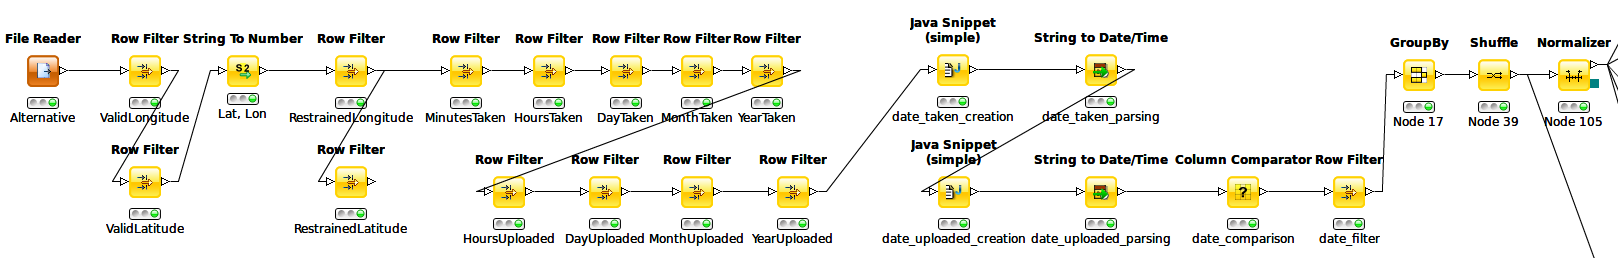
\includegraphics[width=\linewidth]{img/knime_filter.png}
    \caption{Flux de traitement dédié au filtre des données incohérentes}
    \label{knime_filter}
\end{figure}

\subsection{Parsing}
Le parsing des données s'effectue ici à l'aide du composant \textbf{File Reader}, ainsi paramétré :
\begin{itemize}
    \item Column delimiter : ,
    \item Read column headers : true
    \item Ignore spaces and tabs : true
    \item Advanced
    \begin{itemize}
        \item Quote support :
        \begin{itemize}
            \item Quoted strings can extend over multiple lines : true
            \item Quotes characters : \" et '
        \end{itemize}
        \item Ignore spaces : Ignore extra delimiters at end of rows : true
        \item Short lines : Allow short lines : true
        \item Character decoding : ISO-8859-1
    \end{itemize}
\end{itemize}

\subsection{Latitude et longitude}
Un filtre est tout d'abord appliqué sur les colonnes latitude et longitude de type string, à l'aide de deux composants \textbf{Row filter}. Seules les lignes respectant l'expression régulière suivante décrivant un nombre flottant sont alors conservées : $[-]?[0-9]+\backslash.[0-9]+$

Les deux colonnes sont ensuite parsées en nombre grâce au composant \textbf{String to Number}.

Afin de limiter notre étude à la ville de Lyon, et non à ses alentours, ce dans l'optique de rester dans la portée des transports en commun lyonnais, un filtre des composantes latitude et longitude est ensuite appliqué.
On obtient donc grâce à deux composants \textbf{Row Filter} les contraintes suivantes :
\begin{itemize}
    \item $ 4.802508 \leq longitude \leq 4.908976 $
    \item $ 45.715569 \leq latitude \leq 45.793688 $
\end{itemize}

22 782 lignes sont supprimées lors de l'application des filtres sur la latitude et la longitude (60 373 lignes restantes).


\subsection{Champs date et heure}
Afin d'obtenir des données cohérentes vis-à-vis de la date et de l'heure de prise de la photo et de son upload, on applique les contraintes suivantes à l'aide de blocs \textbf{Row Filter} :
\begin{itemize}
    \item $ 0 \leq minutes\_taken \leq 59 $
    \item $ 0 \leq hour\_taken \leq 23 $
    \item $ 1 \leq day\_taken \leq 31 $
    \item $ 1 \leq month\_taken \leq 12 $
    \item $ 2000 \leq year\_taken \leq 2014 $\\

    \item $ 0 \leq hour\_uploaded \leq 23 $
    \item $ 1 \leq day\_uploaded \leq 31 $
    \item $ 1 \leq month\_uploaded \leq 12 $
    \item $ 2000 \leq year\_uploaded \leq 2014 $\\
\end{itemize}

Notons ici que seules les prises effectuées depuis l'an 2000 sont acceptées. On observe en effet que la densité de prise des photos par année augmente fortement dans les années 2000.
Afin de viser les flux touristiques les plus récents, il serait par ailleurs peu intéressant de porter notre étude sur les prises antérieures, exception faite dans un but d'étude de variation des flux touristiques au fil des ans.

225 lignes sont supprimées lors de l'application des filtres sur les champs date et heure des prises et upload de photos (60 148 lignes restantes).\\

Dans un souci de cohérence des données finales, on supprime ensuite toutes les lignes dont la date de prise est postérieure à la date d'upload (notons ici que les champs heure et minute ne sont pas comparés, des conflits dus aux heures locales des appareils photos des touristes et/ou du serveur distant pouvant être observés).

Pour cela deux composants \textbf{Java Snippet} sont utilisés, dans le but de créer deux colonnes (date\_taken et date\_uploaded) contenant un champ date sous forme de String :

\begin{lstlisting}
    return String.format("%d/%d/%d", $day_taken$, $month_taken$, $year_taken$);
\end{lstlisting}

\begin{lstlisting}
    return String.format("%d/%d/%d", $day_uploaded$, $month_uploaded$, $year_uploaded$);
\end{lstlisting}

Deux blocs \textbf{String to Date/Time} permettent alors de transformer au format date les chaînes de caractère initialement de format <dd/MM/yyyy>

Un bloc \textbf{Column Comparator} effectue ensuite la comparaison suivante afin d'initialiser une nouvelle colonne date\_compare :
\begin{lstlisting}
    if(date_uploaded $\heq$ date_taken) {
        date_compare = 'true'
    } else {
        date_compare = 'false'
    }
\end{lstlisting}

Un dernier \textbf{Row Filter} permet enfin de n'accepter que les lignes dont la valeur du champ date\_compare est à "true" .

563 lignes sont supprimées lors du filtre de comparaison des dates de prise et d'upload (59 585 lignes restantes).\\

\subsection{Gestion des doublons}
Afin de supprimer les doublons, un composant \textbf{GroupBy} est enfin appliqué sur la colonne <id>. En ne retenant que les premières valeurs de chaque groupe pour chaque colonne, ce filtre supprime 31 ligne, amenant le nombre de lignes total à 59 554.

\subsection{Mélange}
De par leur complexité, les clustering ultérieurs pourront ne s'appliquer que sur un nombre limité de lignes. Afin d'éviter des résultats faussés par des données non représentatives, le composant \textbf{Shuffle} nous permet ici de mélanger les lignes des données.

\subsection{Normalisation}
Les clustering à venir s'effectuant sur la latitude et la longitude, on normalise ces deux données entre 0 et 1.
\pagebreak



\section{Clustering et évaluation}
Les données étant désormais filtrées, la seconde partie de notre travail réside dans le clustering des données à l'aide d'algorithmes implémentés dans Knime ou dans la librairie SciKit-Learn en Python.

Pour ce faire, différents flux de traitement ont été mis en place, prenant en entrée les données sortant du \textbf{GroupBy} précédemment décrit.

\subsection{K-Means}
\subsubsection{K-Means appliqué à l'ensemble des données}
\begin{figure}[H]
    \centering
    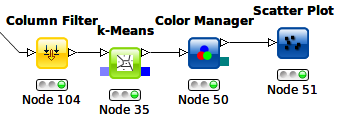
\includegraphics[width=0.5\linewidth]{img/knime_k-means_all.png}
    \caption{Flux de traitement dédié au clustering par K-Means}
\end{figure}

Le composant \textbf{Column Filter} ne conserve que les colonnes latitude et longitude, sur lesquelles sera appliqué le clustering ensuite affiché en fonction de ces deux composantes.

Le composant \textbf{k-Means} est utilisé pour réaliser 60 clusters en un maximum de 99 itérations à partir des colonnes latitude et longitude des données en entrée.

Le nombre de cluster ici utilisé est probablement insuffisant en comparaison du nombre de points d'intérêts potentiel sur Lyon, mais se trouve limité par le bloc \textbf{Color Manager}, lequel est utilisé afin d'assigner une couleur à chaque chaîne de caractère unique de la colonne <cluster> crée par k-means, et ne peut générer automatiquement plus de 60 couleurs pour nos valeurs.
\pagebreak

Le \textbf{Scatter Plot} affiche ensuite les résultats suivants :
\begin{figure}[H]
    \centering
    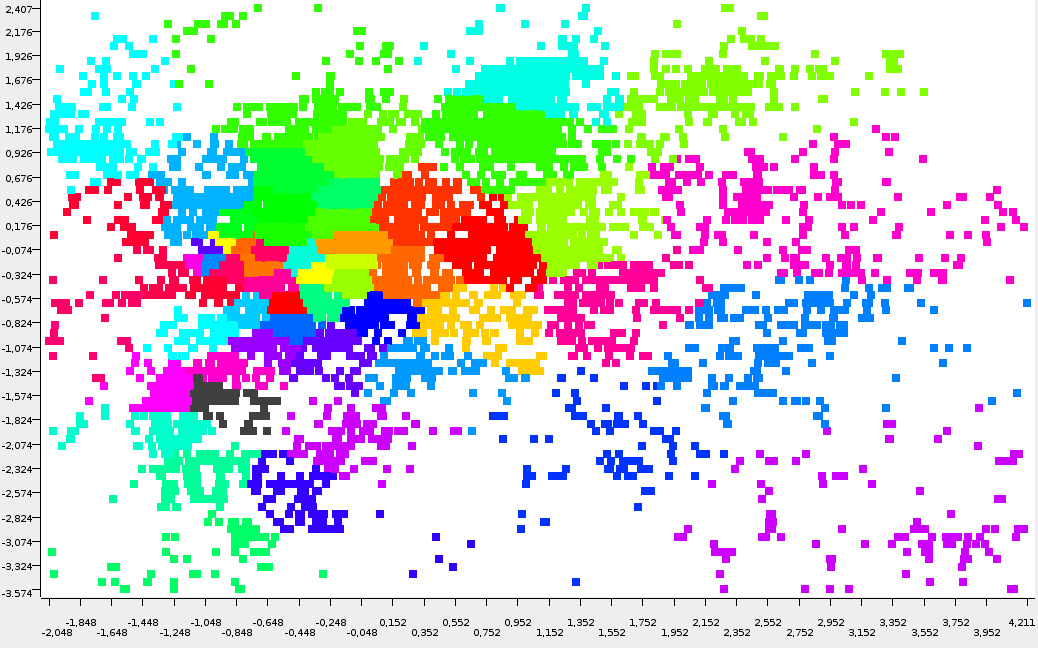
\includegraphics[width=\linewidth]{img/60_means_all.png}
    \caption{Résultats de K-Means, 60 clusters, 59 554 lignes}
\end{figure}

Comme attendu, ces résultats sont peu probants, notamment de par la présence de cluster de très faible densité.

Notons que ce clustering, appliqué sur des données ne restreignant pas la latitude et longitude à la ville de Lyon, donne les résultats suivants :
\begin{figure}[H]
    \centering
    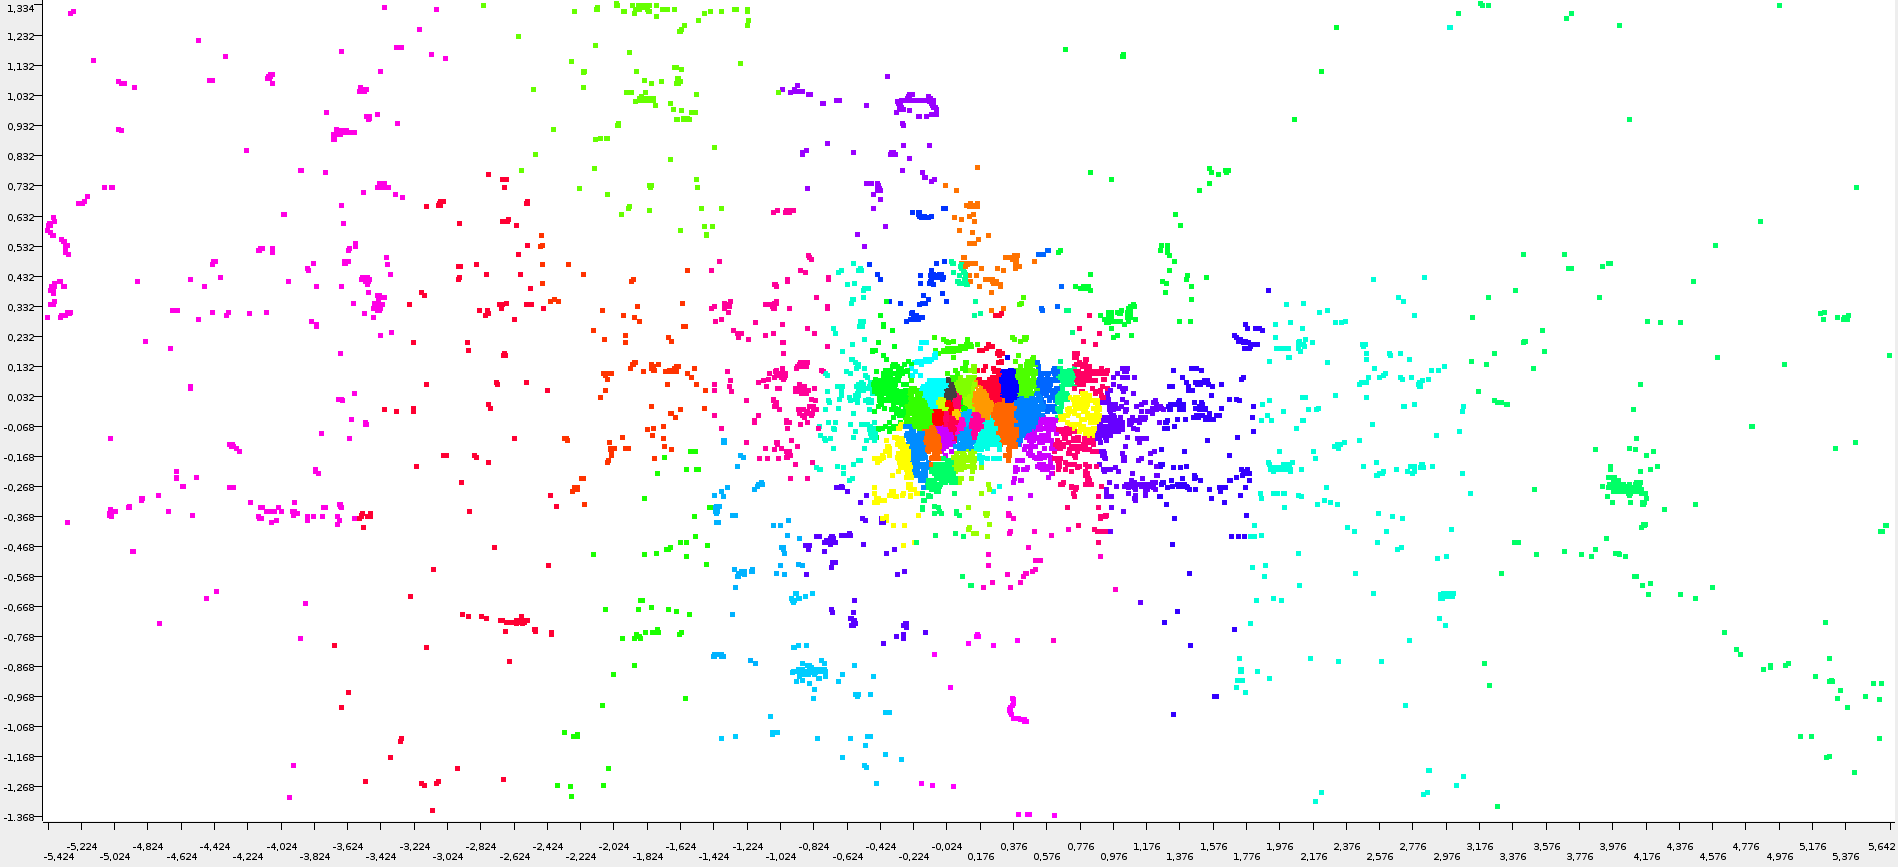
\includegraphics[width=\linewidth]{img/60_means_large.png}
    \caption{Résultats de K-Means, 60 clusters, 82 199 lignes}
\end{figure}

Le nombre de cluster est ici hautement insuffisant au vu du clustering appliqué au centre ville. Les clusters éloignés ne semblent pas non plus pertinents.



\subsubsection{K-Means appliqué aux données de jour}
Une approche de clustering orientée par plages horaire trouve son intérêt vis-à-vis de la gestion des transports en commun. Celle-ci pourrait indiquer les zones à desservir dans un cadre touristique.

En premier lieu, on s'intéressera aux zones d'intérêt de jour, à savoir entre 6h et 21h.

Pour ce faire, le flux de traitement suivant est utilisé :
\begin{figure}[H]
    \centering
    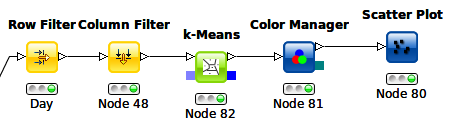
\includegraphics[width=0.8\linewidth]{img/knime_k-means_day.png}
    \caption{Flux de traitement : K-Means appliqué sur une plage horaire de 6h à 21h}
\end{figure}

Un \textbf{Row Filter} a été ajouté au flux de traitement précédent, lequel n'accepte que les lignes dont l'heure de prise se situe entre 6h et 21h.

Les résultats obtenus sont les suivants :
\begin{figure}[H]
    \centering
    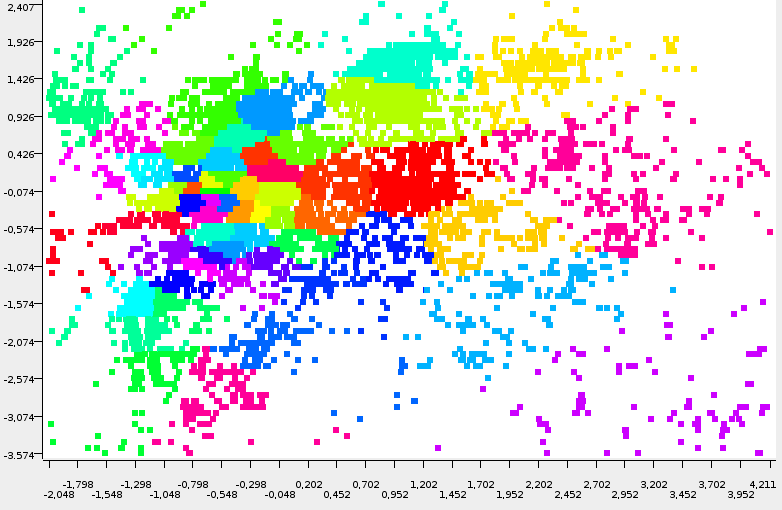
\includegraphics[width=\linewidth]{img/60_means_day.png}
    \caption{Résultats de K-Means, 60 clusters, 47 820 lignes}
\end{figure}

De par le nombre de photos traité extrêmement proche des résultats précédents, peu de différences sont observables. Un tel clustering est peu intéressant.



\subsubsection{K-Means appliqué aux données de nuit}
Les zones d'intérêt de nuit (photos prises de 21h à 6h) peuvent en revanche être davantage exploitées. Pour un flux de traitement identique, le nombre de lignes est bien inférieur (11 734 lignes contre 59 554 initialement).

\begin{figure}[H]
    \centering
    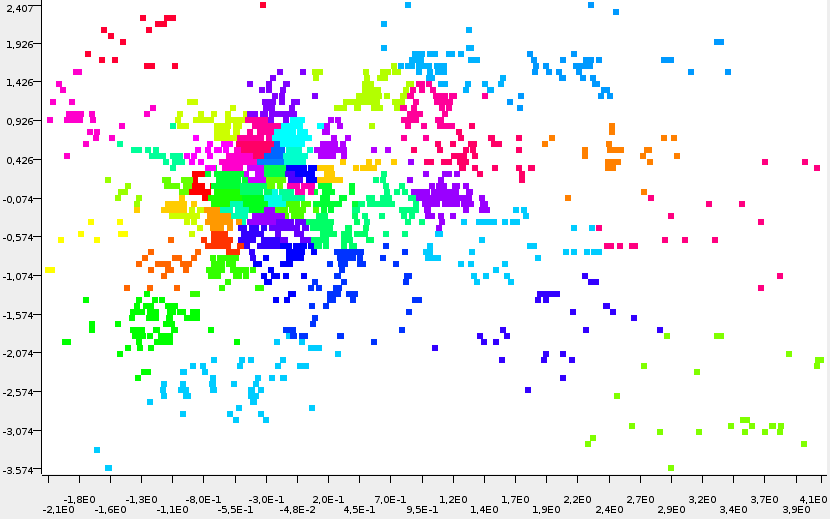
\includegraphics[width=\linewidth]{img/60_means_night.png}
    \caption{Résultats de K-Means, 60 clusters, 11 734 lignes}
\end{figure}

Des différences de cluster peuvent être observées. En effet, les touristes semblent se concentrer sur le Vieux Lyon en ces heures noctures, lequel contient de nombreux bars et restaurants.

Néanmoins, des clusters à faible densité subsistent, et le nombre de cluster présent est toujours probablement insuffisant en comparaison du nombre de points d'intérêt sur Lyon.


\subsection{Étude de K-Means}
K-Means est un algorithme convergeant rapidement et efficace sur des données géolocalisées, notamment dans le cas présent où la répartition des photos est de forme globulaire, celles-ci étant regroupée autour de points d'intérêts.\\

Néanmoins, celui-ci contient néanmoins un certain nombre d'inconvénients.

\begin{itemize}
\item Tout d'abord, le nombre de cluster devant être fixé, cette contrainte s'oppose ici à l'évaluation du nombre de points d'intérêts sur Lyon, ce nombre faisant justement parti des données recherchées.

\item Par ailleurs, K-means inclut le bruit dans son clustering, d'où la présence de cluster de faible densité, ne comportant parfois aucun point d'intérêt manifeste.

\item Enfin, les limites de cet algorithme sont ici illustrées dans le cas de clusters de taille et de densité différente. Dans le cas du centre de Lyon par exemple, il s'agît d'un cluster de grande taille, et de densité variable. K-means est peu efficace et regroupe ici de nombreux points d'intérêt en un seul.\item
\end{itemize}

Une approche par densité semble donc d'intérêt, et sera effectuée ultérieurement.

\pagebreak



\subsection{Clustering hiérarchique}
Une approche par clustering hiérarchique est également envisageable. Néanmoins, de par le temps requis par ce clustering, un échantillonnage à hauteur de 1 000 photos est ici utilisé.

\begin{figure}[H]
    \centering
    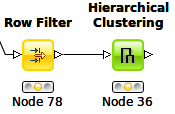
\includegraphics[width=0.25\linewidth]{img/knime_hierarchical.png}
    \caption{Flux de traitement : Clustering hiérarchique sur 1 000 photos}
\end{figure}

Le clustering hiérarchique s'effectue sur la latitude et longitude, pour 90 clusters en sortie, la distance Euclidienne étant utilisée.

Les résultats obtenus sont les suivants :
\begin{figure}[H]
    \centering
    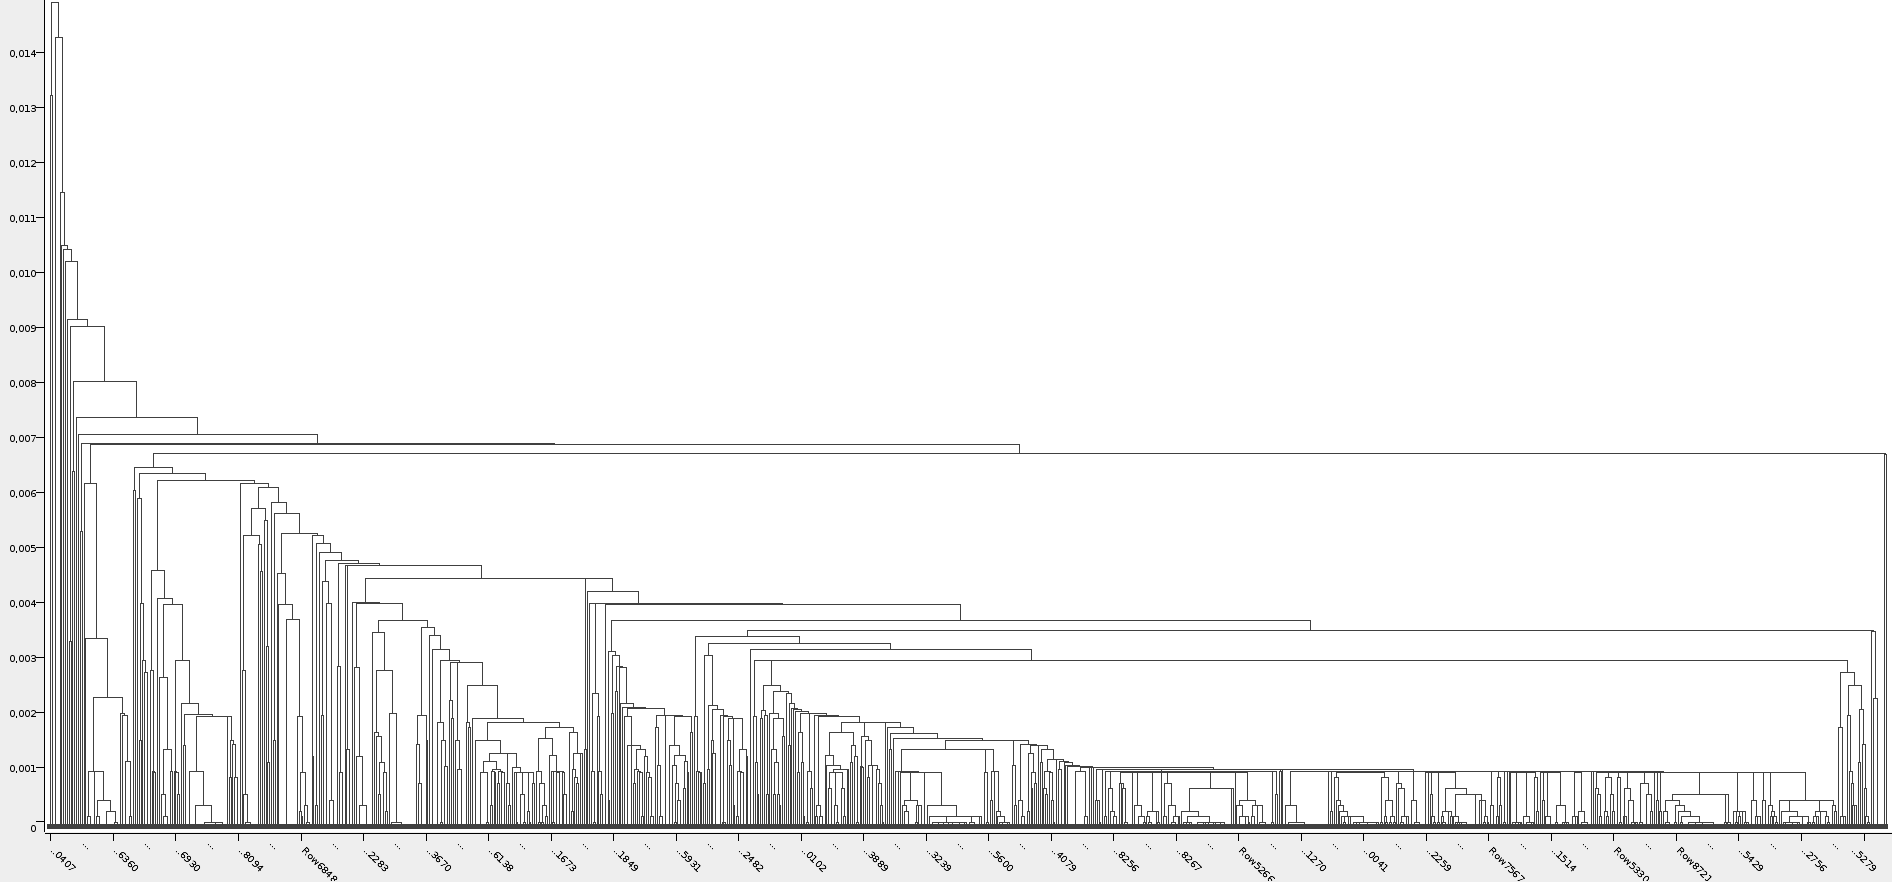
\includegraphics[width=\linewidth]{img/1000_histo1.png}
    \caption{Dendrogramme pour 1 000 lignes}
\end{figure}

\begin{figure}[H]
    \centering
    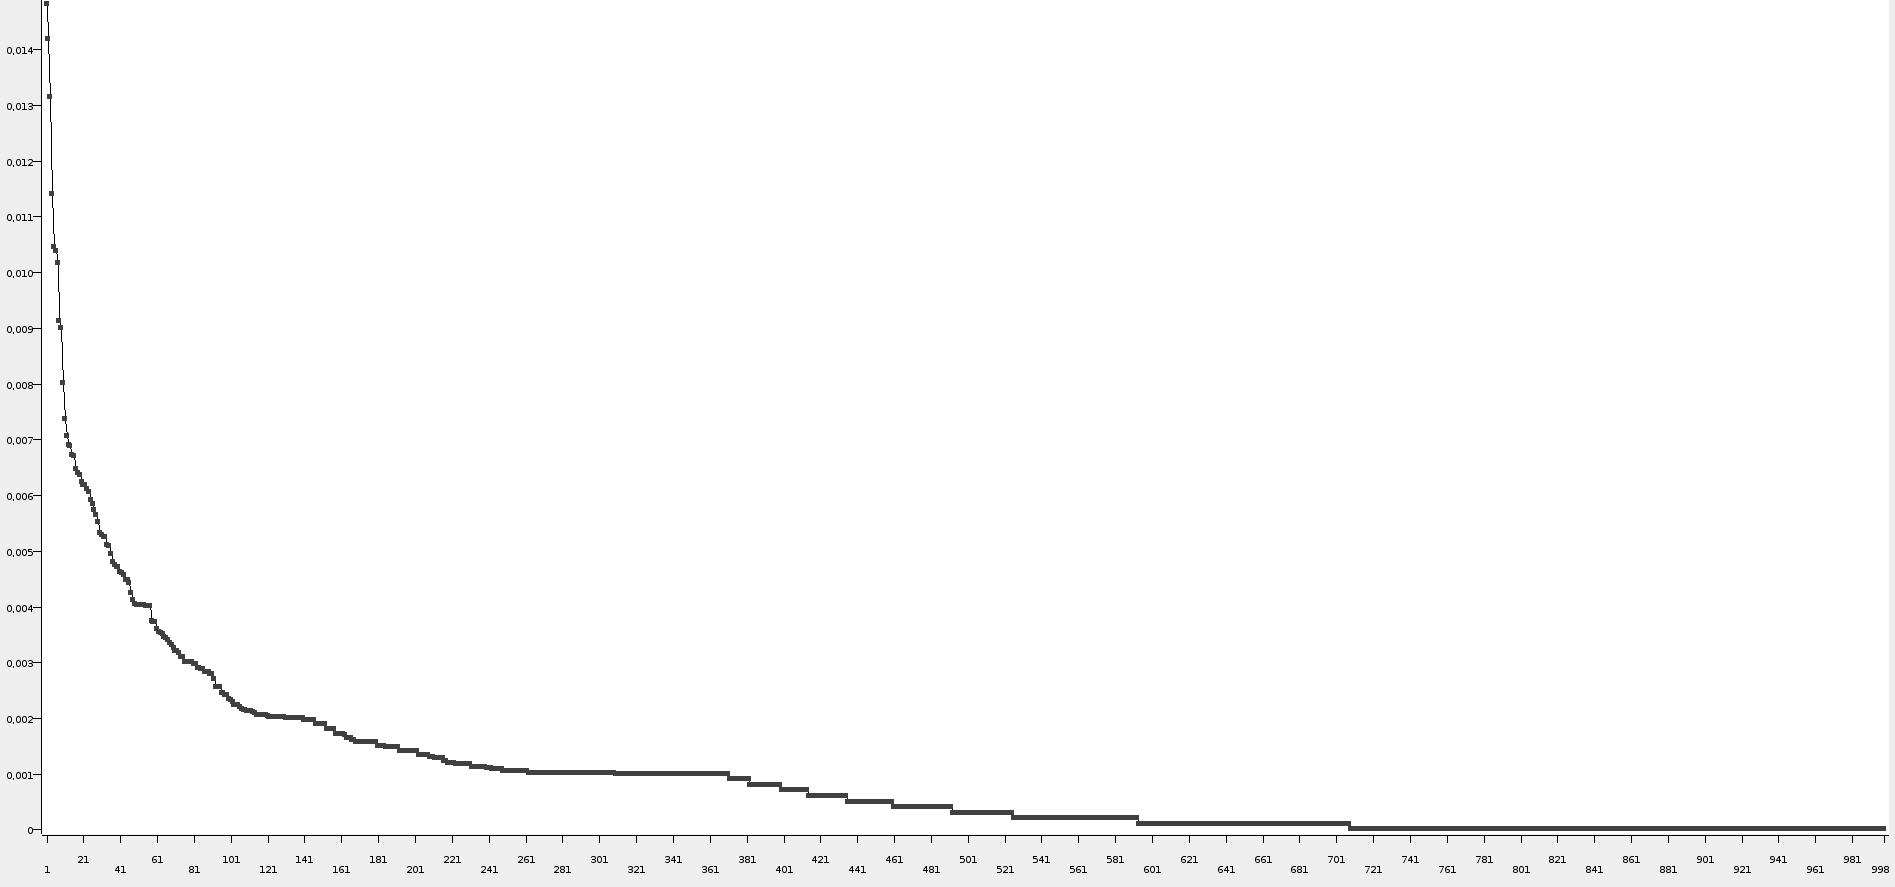
\includegraphics[width=\linewidth]{img/1000_histo2.png}
    \caption{Distance entre les clusters pour 1 000 lignes}
\end{figure}

hierarchical : permet de choisir nbclusters, mais echantillonnage
choisir centroides puis donnner à K-means

Si l'on observe des regroupements certains, avec des clusters d'une intéressante densité, le choix du seuil de coupe de l'arbre du dendrogramme n'est pas aisé, la hauteur des clustering de densité variant fortement.
Le choix du nombre de cluster est donc ici encore nécessaire, inconvénient dans le cas où l'un des buts du clustering est de déterminer le nombre et l'identité des points d'intérêt. Malgré un \textit{shuffle}, l'échantillonnage n'est par ailleurs pas forcément représentatif.

Toutefois, une approche intéressante pourrait être de déterminer un ensemble de centroïdes basé sur une étude dudit dendrogramme, puis d'utiliser ceux-ci comme centroïdes initiaux pour l'algorithmes K-means. Les résultats dégagés par K-means pourraient alors en être améliorés.
\pagebreak



\subsection{DBSCAN}
Une approche par densité est à présent effectuée, utilisant l'algorithme DBSCAN.
Rappelons que DBScan utilise deux paramètres afin de calculer des clusters, que sont une distance epsilon, et un nombre minimum de point MinPoints. Le fonctionnement de cet algorithme repose sur ce principe : on recherche les points dont les voisins à une distance inférieur à espilon sont au moins au nombre de minPoint. On part d'un point, et on cherche ainsi tous les points qui sont ses voisins, auquel on applique l'algorithme jusqu'à ne plus avoir assez de voisins. Les points parcourus et vérifiants le nombre de voisins minimum feront alors partie du même cluster.

Il est intéressant d'amener une première reflexion quant à l'efficacité de notre DBScan dès lors que nous avons les informations sur son algorithme de calcul. Si on fixe une valeur d'epsilon très faible, nous pourrons discerner des clusters dans un amas de point à forte densité. Si un autre amas possède une densité plus faible, le cluster risque d'être effacé du fait qu'il n'y aura pas minpoints au voisinage d'un point. On pourrait alors augmenter la valeur d'epsilon, mais de nouveau, nous nous retrouvons face à un poblème. A l'inverse, cette fois-ci, les zones à très forte densité ne formeront qu'un cluster car tous les points seront assez proches les uns des autres pour être en dessous de la barre de epsilon.
Nous allons donc voir si il est possible de concillier ces deux points afin d'obtenir un clustering correct. 

\begin{figure}[H]
    \centering
    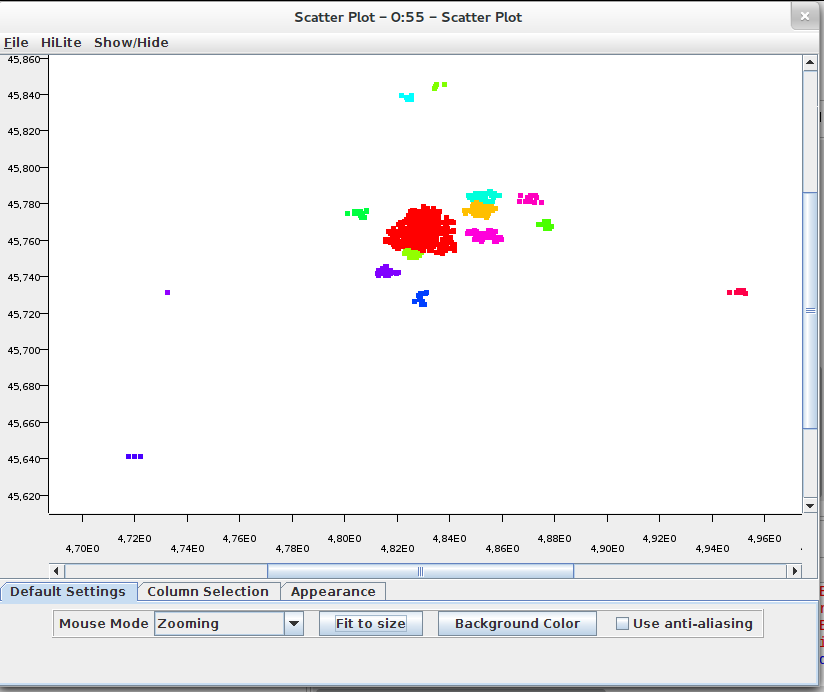
\includegraphics[width=\linewidth]{img/dbscan_50.png}
    \caption{Lalalilu}
\end{figure}

Nous obtenons tout d'abord un premier résultat satisfaisant, mais seulement pour les clusters externes à ce qu'on pourrait identifier comme le centre de lyon au vu de la densité de photos. En effet, on observe dans le périphérique du grand lyon des clusters bien identifiés, mais un seul cluster est identifié pour l'ensemble des points apparaissants au centre de l'image. Ce n'est pas ce que nous cherchons. Il faut alors affiner la distance, afin de pouvoir les séparer et obtenir des clusters plus fins .

\begin{figure}[H]
    \centering
    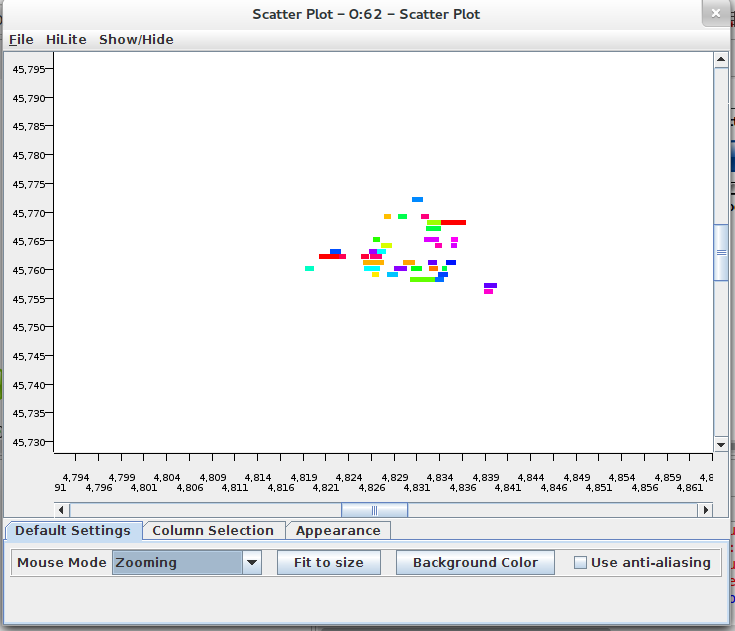
\includegraphics[width=\linewidth]{img/dbscan_21.png}
    \caption{Lalalilu}
\end{figure}


Afin d'éviter de perdre les clusters de l'extérieur, il nous suffit de récupérer le cluster central, et de lui ré-appliquer DBScan, avec cette fois ci des valeurs plus fines. Nous obtenons alors le résultat précédent, sur lequel on observe des clusters intéressants !
Cela donne sous Knime un schéma de cette forme :

\begin{figure}[H]
    \centering
    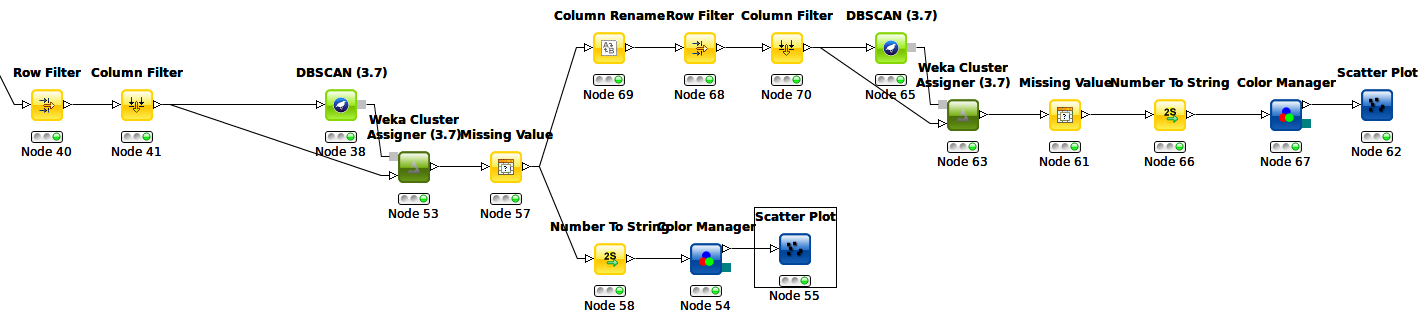
\includegraphics[width=\linewidth]{img/knime_dbscan.png}
    \caption{Flux de traitement : Clustering par DBSCAN}
\end{figure}

Il faudrait dans l'idéal rediriger les deux sorties vers la même table, mais après quelques essaies non-fructueux, nous avons préféré en rester là, et se centrer sur K-Means pour la partie de visualisation.
Nous pouvons conclure, comme vu dans le cours, que DBScan n'est pas performant pour identifier des clusters sur des données à densité variable, comme c'est le cas ici entre le centre de lyon et le périphérique.

\pagebreak




\subsection{Mean Shift}
Souhaitant expérimenter l'algorithme Mean Shift, utilisant une approche du clustering par densité, nous exportons à présent l'ensemble des données nettoyées et filtrées au format CSV.

\subsubsection{Export des données}
Cet export se situe entre le bloc \textbf{Shuffle} et \textbf{Normalizer} (Voir \ref{knime_filter}).

\begin{figure}[H]
    \centering
    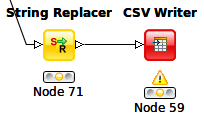
\includegraphics[width=0.25\linewidth]{img/knime_csvwriter.png}
    \caption{Flux de traitement : Export des données au format CSV sous Knime}
\end{figure}

Le composant \textbf{String Replacer} permet de transformer les caractères $'\backslash n'$ en la suite de caractères $'\backslash \backslash n'$ dans le champ <legend> (utilisation d'une expression régulière).

L'ensemble des données est ensuite exporté par le composant \textbf{CSV Writer}.

\subsubsection{Mean Shift en Python}
La librairie open source d'analyse de données \textbf{Pandas} a tout d'abord été utilisée afin de réaliser le parsing du document CSV et la manipulation de la matrice de données obtenue.

L'algorithme \textbf{Mean Shift} de la librairie Python \textbf{SciKit-Learn} est ensuite appliqué sur la latitude et longitude, les données étant filtrées au préalable par Knime.pour la construction d'une estimation nommée \textit{bandwidth}. Paramètres :
\begin{itemize}
    \item quantile : 0.005
    \item n\_samples : None
\end{itemize}

Une instance de la classe MeanShift est ensuite crée à l'aide de l'estimation bandwidth précédente et des paramètres suivants :
\begin{itemize}
    \item bin\_seeding : True
    \item min\_bin\_freq : 30
    \item cluster\_all : False
\end{itemize}

On supprime alors tous les clusters dont le nombre de points est inférieur à 30. La suppression du bruit et le filtre de nombre de points par cluster restreint le nombre de photos qui était initialement de 59 554 à 47 800.
Les résultats suivants sont obtenusy :
\begin{figure}[H]
    \centering
    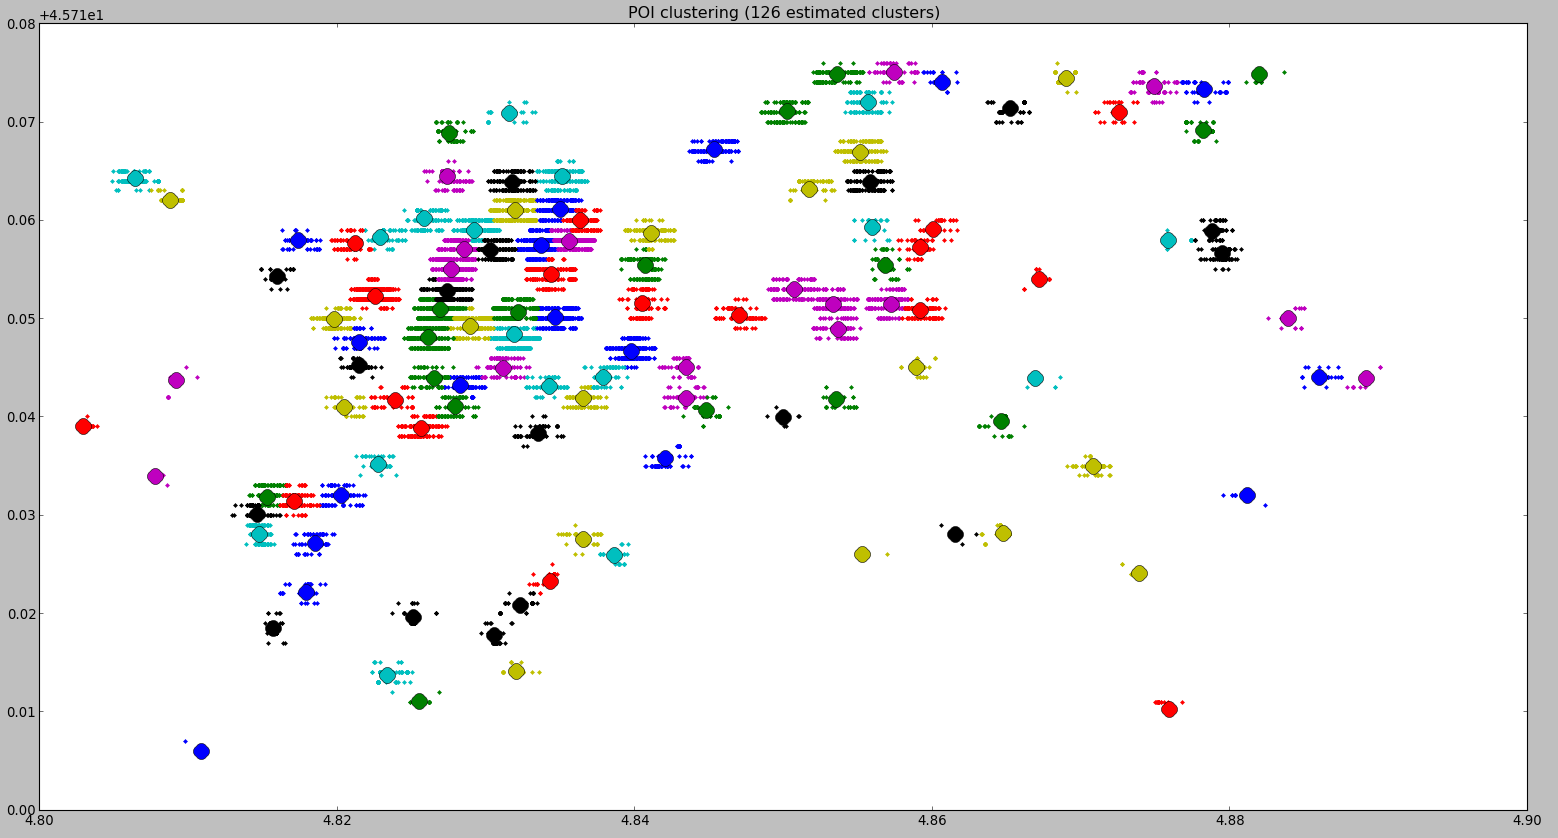
\includegraphics[width=\linewidth]{img/meanshift.png}
    \caption{Résultats du clustering par Mean Shift, 126 clusters, 47 800 photos}
\end{figure}

Comme on peut l'observer, l'approche par densité donne de bien meilleurs résultats. Le bruit n'est pas ici clusterisé et a été éliminé des résultats. Seuls les clusters de densité suffisante et ayant un certain nombre de points sont alors conservés. Toutefois, la validité de ce clustering devrait encore être vérifiée à l'aide d'outils tels Google Places.


Au vu des résultats probants précédents, des clustering plus affinés peuvent également être envisagés. Ci-dessous, les points d'intérêts correspondant aux prises de photos réalisées entre le 6 et 9 Décembre inclus, ces dates correspondant à la Fête des Lumières sur Lyon, et de ce fait à un pic massif d'utilisation des transports en commun.
\begin{figure}[H]
    \centering
    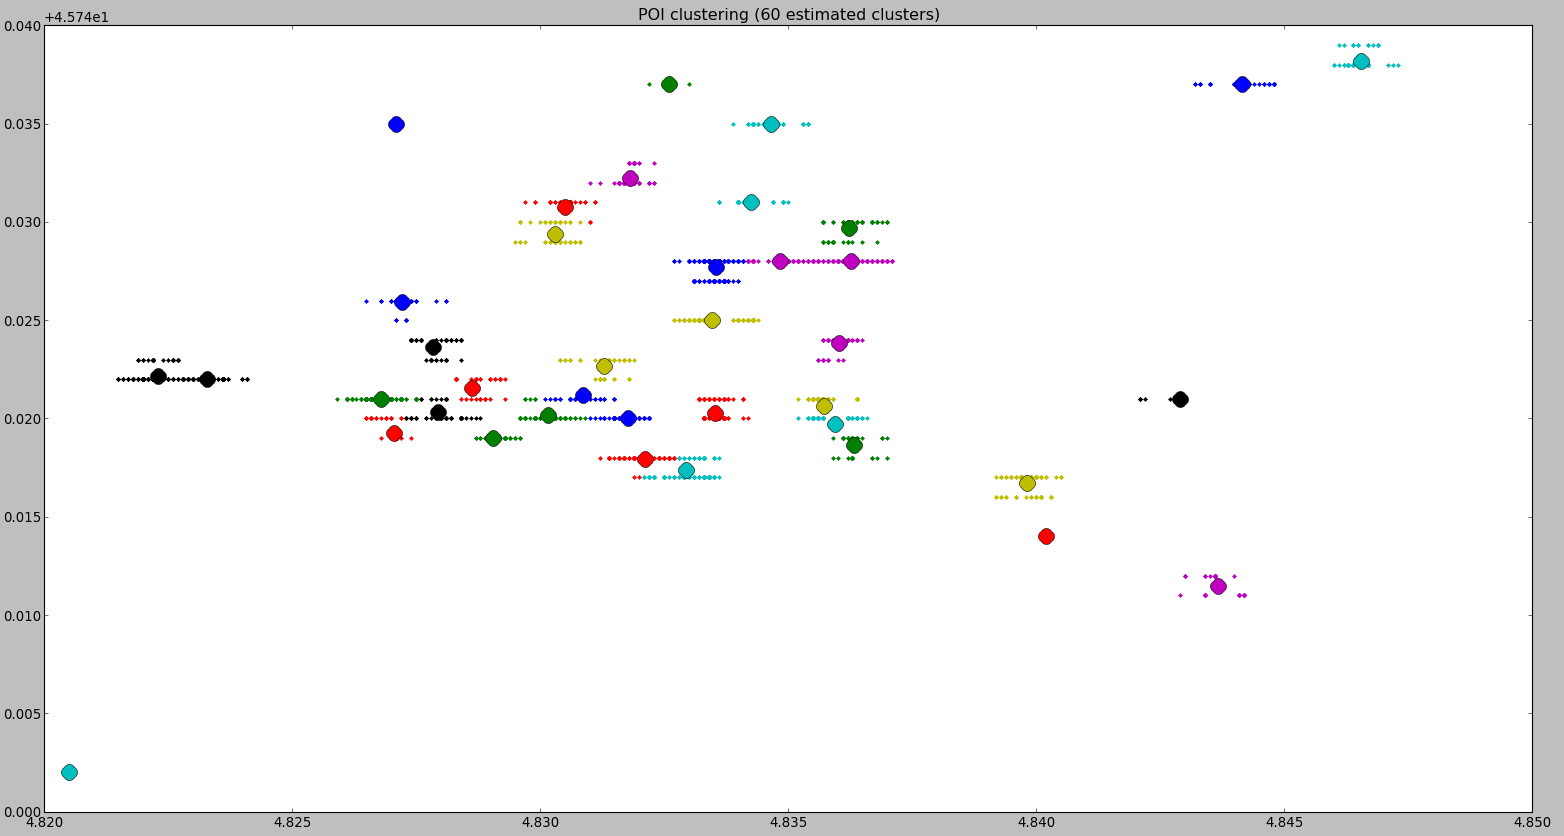
\includegraphics[width=\linewidth]{img/meanshift_lumieres.png}
    \caption{Résultats du clustering par Mean Shift, 60 clusters, 4 100 photos}
\end{figure}

Un rapprochement entre ces zones et les arrêts TCL les plus proches permettrait d'optimiser le désservissement des zones les plus visitées à cette époque de l'année.

Le résultat de ces clustering est enfin exporté au format CSV afin d'être affiché grâce à un serveur Web.
\pagebreak



\section{Visualisation des résultats}

\pagebreak


\section{Description des clusters}
TODO : Google Places ?
\pagebreak


\section{Something ?}
On a fait des trucs en plus ?
- Détecter les évènements basés sur une date
- Etudier la variation des flux touristiques au fil des ans
=> Passage à l’échelle ? Tâches prédictives ? Analyse dynamique et non statique ? Autres sources ? (Tweets, Instagram,…)
\pagebreak
